% =============================================================================
% UNet Architecture Diagram — Caries Segmentation Project
% =============================================================================
% Input : 3 × 384 × 384   |   Output: 1 × 384 × 384
% Filters: [64, 128, 256, 512, 1024]
% =============================================================================
\documentclass[border=5pt]{standalone}
\usepackage{tikz}
\usepackage{xcolor}
\usetikzlibrary{arrows.meta, positioning, calc, decorations.pathreplacing}

% ---------------------------------------------------------------------------
% Color palette
% ---------------------------------------------------------------------------
\definecolor{convblue}{RGB}{100, 149, 237}      % Conv blocks (encoder)
\definecolor{convbluelight}{RGB}{173, 199, 245}  % Conv blocks (decoder)
\definecolor{poolred}{RGB}{220, 80, 60}          % MaxPool arrows
\definecolor{upgreen}{RGB}{60, 179, 113}         % UpConv arrows
\definecolor{skipgray}{RGB}{180, 180, 180}       % Skip connections
\definecolor{outputyellow}{RGB}{255, 193, 37}    % 1×1 Conv / output
\definecolor{catpurple}{RGB}{155, 89, 182}       % Concatenation arrows
\definecolor{bottleneck}{RGB}{70, 130, 180}      % Bottleneck block

% ---------------------------------------------------------------------------
% Styles
% ---------------------------------------------------------------------------
\tikzset{
    % Encoder conv block
    encblock/.style={
        draw=convblue!80!black, thick,
        fill=convblue!25,
        minimum width=#1,        % proportional to spatial size
        minimum height=0.7cm,
        rounded corners=2pt,
        font=\footnotesize\sffamily,
        inner sep=3pt,
    },
    % Decoder conv block
    decblock/.style={
        draw=convbluelight!80!black, thick,
        fill=convbluelight!40,
        minimum width=#1,
        minimum height=0.7cm,
        rounded corners=2pt,
        font=\footnotesize\sffamily,
        inner sep=3pt,
    },
    % Bottleneck block
    bnblock/.style={
        draw=bottleneck!80!black, thick,
        fill=bottleneck!30,
        minimum width=#1,
        minimum height=0.7cm,
        rounded corners=2pt,
        font=\footnotesize\sffamily,
        inner sep=3pt,
    },
    % Output block
    outblock/.style={
        draw=outputyellow!80!black, thick,
        fill=outputyellow!35,
        minimum width=#1,
        minimum height=0.7cm,
        rounded corners=2pt,
        font=\footnotesize\sffamily,
        inner sep=3pt,
    },
    % Input block
    inblock/.style={
        draw=black!60, thick,
        fill=black!8,
        minimum width=#1,
        minimum height=0.7cm,
        rounded corners=2pt,
        font=\footnotesize\sffamily,
        inner sep=3pt,
    },
    % Down arrow (MaxPool)
    downarrow/.style={
        -{Stealth[length=4pt]},
        thick,
        poolred,
    },
    % Up arrow (UpConv)
    uparrow/.style={
        -{Stealth[length=4pt]},
        thick,
        upgreen,
    },
    % Skip connection
    skiparrow/.style={
        -{Stealth[length=4pt]},
        thick,
        skipgray,
        dashed,
    },
    % Conv arrow (within same level)
    convarrow/.style={
        -{Stealth[length=3pt]},
        thick,
        black!60,
    },
    % Label style
    dimlabel/.style={
        font=\scriptsize\sffamily,
        text=black!70,
    },
    % Channel label style
    chlabel/.style={
        font=\scriptsize\sffamily\bfseries,
        text=black!90,
    },
    % Operation label style
    oplabel/.style={
        font=\tiny\sffamily,
        text=black!60,
        fill=white,
        fill opacity=0.8,
        text opacity=1,
        inner sep=1pt,
        rounded corners=1pt,
    },
}

\begin{document}
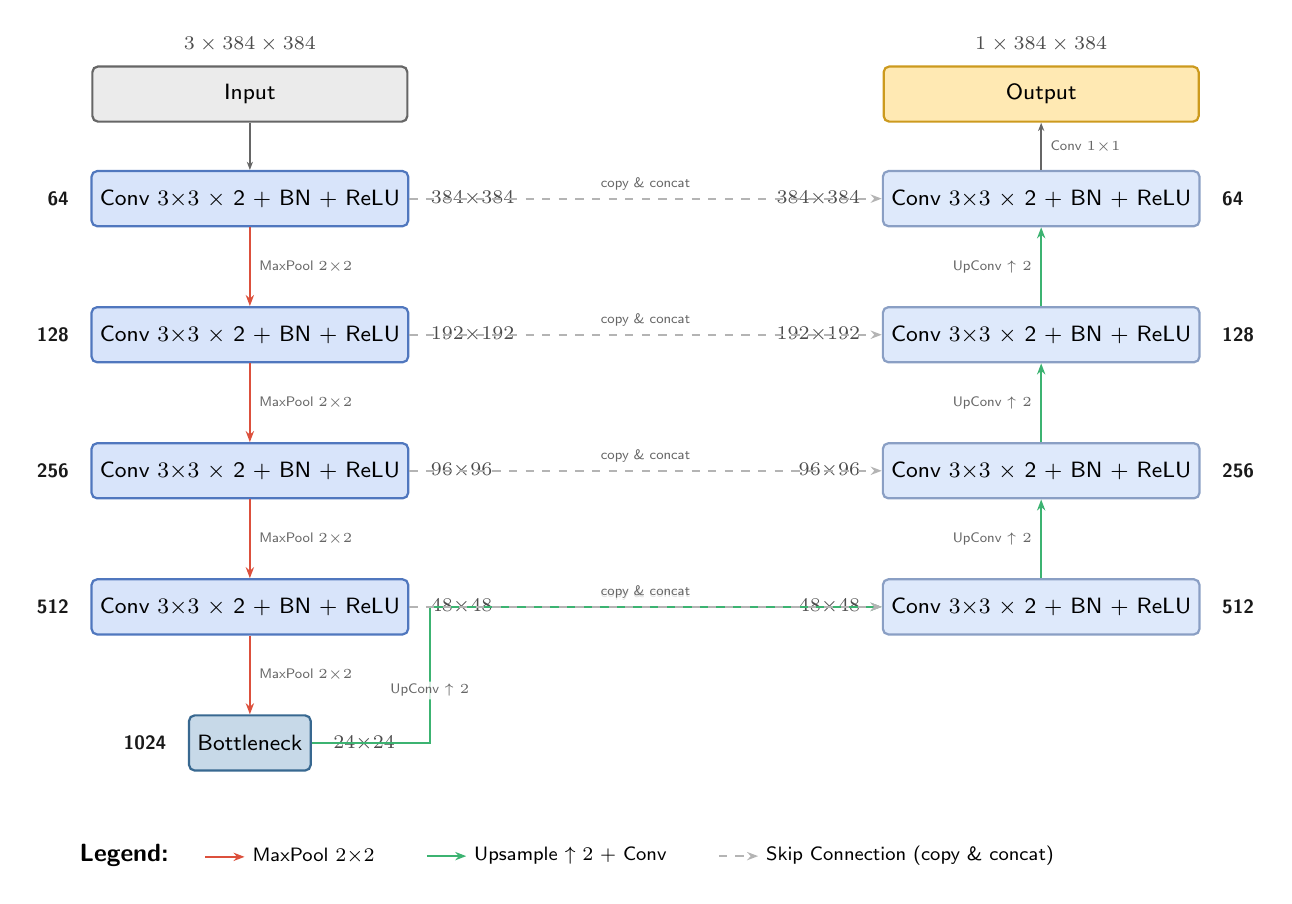
\begin{tikzpicture}[node distance=0.5cm]

% =========================================================================
% Block widths proportional to spatial resolution
% 384 -> 4.0cm,  192 -> 3.0cm,  96 -> 2.2cm,  48 -> 1.6cm,  24 -> 1.2cm
% =========================================================================

% =========================================================================
% ENCODER (left side, going down)
% =========================================================================

% --- Input ---
\node[inblock=4.0cm] (input) {Input};
\node[dimlabel, above=0.05cm of input] {$3 \times 384 \times 384$};

% --- Encoder Level 1: 64 × 384 × 384 ---
\node[encblock=4.0cm, below=0.6cm of input] (e1) {Conv $3{\times}3$ $\times$ 2 + BN + ReLU};
\node[chlabel, left=0.15cm of e1] {64};
\node[dimlabel, right=0.15cm of e1] {$384{\times}384$};

% --- Encoder Level 2: 128 × 192 × 192 ---
\node[encblock=3.0cm, below=1.0cm of e1] (e2) {Conv $3{\times}3$ $\times$ 2 + BN + ReLU};
\node[chlabel, left=0.15cm of e2] {128};
\node[dimlabel, right=0.15cm of e2] {$192{\times}192$};

% --- Encoder Level 3: 256 × 96 × 96 ---
\node[encblock=2.2cm, below=1.0cm of e2] (e3) {Conv $3{\times}3$ $\times$ 2 + BN + ReLU};
\node[chlabel, left=0.15cm of e3] {256};
\node[dimlabel, right=0.15cm of e3] {$96{\times}96$};

% --- Encoder Level 4: 512 × 48 × 48 ---
\node[encblock=1.6cm, below=1.0cm of e3] (e4) {Conv $3{\times}3$ $\times$ 2 + BN + ReLU};
\node[chlabel, left=0.15cm of e4] {512};
\node[dimlabel, right=0.15cm of e4] {$48{\times}48$};

% --- Bottleneck: 1024 × 24 × 24 ---
\node[bnblock=1.2cm, below=1.0cm of e4] (e5) {Bottleneck};
\node[chlabel, left=0.15cm of e5] {1024};
\node[dimlabel, right=0.15cm of e5] {$24{\times}24$};

% =========================================================================
% DECODER (right side, going up)
% =========================================================================

% --- Decoder Level 5: 512 × 48 × 48 ---
\node[decblock=1.6cm, right=6.0cm of e4] (d5) {Conv $3{\times}3$ $\times$ 2 + BN + ReLU};
\node[chlabel, right=0.15cm of d5] {512};
\node[dimlabel, left=0.15cm of d5] {$48{\times}48$};

% --- Decoder Level 4: 256 × 96 × 96 ---
\node[decblock=2.2cm, above=1.0cm of d5] (d4) {Conv $3{\times}3$ $\times$ 2 + BN + ReLU};
\node[chlabel, right=0.15cm of d4] {256};
\node[dimlabel, left=0.15cm of d4] {$96{\times}96$};

% --- Decoder Level 3: 128 × 192 × 192 ---
\node[decblock=3.0cm, above=1.0cm of d4] (d3) {Conv $3{\times}3$ $\times$ 2 + BN + ReLU};
\node[chlabel, right=0.15cm of d3] {128};
\node[dimlabel, left=0.15cm of d3] {$192{\times}192$};

% --- Decoder Level 2: 64 × 384 × 384 ---
\node[decblock=4.0cm, above=1.0cm of d3] (d2) {Conv $3{\times}3$ $\times$ 2 + BN + ReLU};
\node[chlabel, right=0.15cm of d2] {64};
\node[dimlabel, left=0.15cm of d2] {$384{\times}384$};

% --- Output ---
\node[outblock=4.0cm, above=0.6cm of d2] (output) {Output};
\node[dimlabel, above=0.05cm of output] {$1 \times 384 \times 384$};

% =========================================================================
% ARROWS — Encoder (down)
% =========================================================================
\draw[convarrow] (input) -- (e1);

\draw[downarrow] (e1) -- node[oplabel, right=2pt] {MaxPool $2{\times}2$} (e2);
\draw[downarrow] (e2) -- node[oplabel, right=2pt] {MaxPool $2{\times}2$} (e3);
\draw[downarrow] (e3) -- node[oplabel, right=2pt] {MaxPool $2{\times}2$} (e4);
\draw[downarrow] (e4) -- node[oplabel, right=2pt] {MaxPool $2{\times}2$} (e5);

% =========================================================================
% ARROWS — Bottleneck to Decoder
% =========================================================================
% Bottleneck → UpConv → d5
\draw[uparrow] (e5.east) -- ++(1.5,0) |- node[oplabel, pos=0.25, below=2pt] {UpConv $\uparrow 2$} (d5.west);

% =========================================================================
% ARROWS — Decoder (up)
% =========================================================================
\draw[uparrow] (d5) -- node[oplabel, left=2pt] {UpConv $\uparrow 2$} (d4);
\draw[uparrow] (d4) -- node[oplabel, left=2pt] {UpConv $\uparrow 2$} (d3);
\draw[uparrow] (d3) -- node[oplabel, left=2pt] {UpConv $\uparrow 2$} (d2);

% Output 1×1 conv
\draw[convarrow] (d2) -- node[oplabel, right=2pt] {Conv $1{\times}1$} (output);

% =========================================================================
% SKIP CONNECTIONS (encoder → decoder)
% =========================================================================
\draw[skiparrow] (e4.east) -- node[oplabel, above=1pt] {copy \& concat} (d5.west |- e4.east);
% We need to draw them properly: horizontal lines from encoder to decoder

% e4 → d5 (same vertical level)
\draw[skiparrow] (e4.east) -- (d5.west);
\node[oplabel] at ($(e4.east)!0.5!(d5.west)$) [above=2pt] {copy \& concat};

% e3 → d4
\draw[skiparrow] (e3.east) -- (d4.west);
\node[oplabel] at ($(e3.east)!0.5!(d4.west)$) [above=2pt] {copy \& concat};

% e2 → d3
\draw[skiparrow] (e2.east) -- (d3.west);
\node[oplabel] at ($(e2.east)!0.5!(d3.west)$) [above=2pt] {copy \& concat};

% e1 → d2
\draw[skiparrow] (e1.east) -- (d2.west);
\node[oplabel] at ($(e1.east)!0.5!(d2.west)$) [above=2pt] {copy \& concat};

% =========================================================================
% LEGEND
% =========================================================================
\node[anchor=north west, font=\small\sffamily\bfseries] at ($(e5.south west) + (-1.5, -0.8)$) (legendtitle) {Legend:};

\node[right=0.2cm of legendtitle, anchor=west, font=\scriptsize\sffamily] (leg1) {%
    \tikz{\draw[downarrow] (0,0) -- (0.5,0);} MaxPool $2{\times}2$};

\node[right=0.4cm of leg1, anchor=west, font=\scriptsize\sffamily] (leg2) {%
    \tikz{\draw[uparrow] (0,0) -- (0.5,0);} Upsample $\uparrow 2$ + Conv};

\node[right=0.4cm of leg2, anchor=west, font=\scriptsize\sffamily] (leg3) {%
    \tikz{\draw[skiparrow] (0,0) -- (0.5,0);} Skip Connection (copy \& concat)};

\end{tikzpicture}
\end{document}
